\documentclass[master=elt,masteroption=ec,english]{kulemt}
\setup{
  title={The best master's thesis ever},
  author={Een Auteur\and Tweede Auteur},
  promotor={Prof.\,dr.\,ir.\ Weet Beter},
  assessor={Ir.\,W. Eetveel\and W. Eetrest},
  assistant={Ir.\ A.~Assistent \and D.~Vriend}}
% Verwijder de "%" op de volgende lijn als je de kaft wil afdrukken
%\setup{coverpageonly}
% Verwijder de "%" op de volgende lijn als je enkel de eerste pagina's wil
% afdrukken en de rest bv. via Word aanmaken.
%\setup{frontpagesonly}

% Hier kun je dan nog andere pakketten laden of eigen definities voorzien

% Tenslotte wordt hyperref gebruikt voor pdf bestanden.
% Dit mag verwijderd worden voor de af te drukken versie.
\usepackage[pdfusetitle,colorlinks,plainpages=false]{hyperref}

%%%%%%%
% Om wat tekst te genereren wordt hier het lipsum pakket gebruikt.
% Bij een echte masterproef heb je dit natuurlijk nooit nodig!
\IfFileExists{lipsum.sty}%
 {\usepackage{lipsum}\SetLipsumDefault{11-13}}%
 {\newcommand{\lipsum}[1][11-13]{\par Hier komt wat tekst: lipsum ##1.\par}}
%%%%%%%

%\includeonly{chapter-n}
\begin{document}

\begin{preface}
  I would like to thank everybody who kept me busy the last year,
  especially my promoter and my assistants. I would also like to thank the
  jury for reading the text. My sincere gratitude also goes to my wive and
  the rest of my family.
\end{preface}

\tableofcontents*

\begin{abstract}
  The \texttt{abstract} environment contains a more extensive overview of
  the work. But it should be limited to one page.

  \lipsum[1]
\end{abstract}

\begin{abstract*}
  In dit \texttt{abstract} environment wordt een al dan niet uitgebreide
  Nederlandse samenvatting van het werk gegeven.
  Wanneer de tekst voor een Nederlandstalige master in het Engels wordt
  geschreven, wordt hier normaal een uitgebreide samenvatting verwacht,
  bijvoorbeeld een tiental bladzijden. 

  \lipsum[1]
\end{abstract*}

% Een lijst van figuren en tabellen is optioneel
%\listoffigures
%\listoftables
% Bij een beperkt aantal figuren en tabellen gebruik je liever het volgende:
\listoffiguresandtables
% De lijst van symbolen is eveneens optioneel.
% Deze lijst moet wel manueel aangemaakt worden, bv. als volgt:
\chapter{List of Abbreviations and Symbols}
\section*{Abbreviations}
\begin{flushleft}
  \renewcommand{\arraystretch}{1.1}
  \begin{tabularx}{\textwidth}{@{}p{12mm}X@{}}
    LoG   & Laplacian-of-Gaussian \\
    MSE   & Mean Square error \\
    PSNR  & Peak Signal-to-Noise ratio \\
  \end{tabularx}
\end{flushleft}
\section*{Symbols}
\begin{flushleft}
  \renewcommand{\arraystretch}{1.1}
  \begin{tabularx}{\textwidth}{@{}p{12mm}X@{}}
    42    & ``The Answer to the Ultimate Question of Life, the Universe,
            and Everything'' according to \cite{h2g2} \\
    $c$   & Speed of light \\
    $E$   & Energy \\
    $m$   & Mass \\
    $\pi$ & The number pi \\
  \end{tabularx}
\end{flushleft}

% Nu begint de eigenlijke tekst
\mainmatter

\chapter{Introduction}
\label{cha:intro}
The first contains a general introduction to the work. The goals are
defined and the modus operandi is explained.

\section{The problem}
TEEs can be used for 

\section{Paper outline}
\begin{itemize}
    \item Schetsing van het probleem: Wat is het probleem, wat zijn de extra moeilijkheden ivm IoT, OTA update security schetsen in wijdere wereld van IoT security
    \item Beschrijving van huidige literatuur en verwante security oplossingen
    \item Hoog-level beschrijving van oplossing, technisch 
    \item Implementatie mbv board 
\end{itemize}

\section{Trusted Execution Environments: A Technical Overview of Intel SGX, Arm TrustZone, and RISC-V PMP}
\hyperlink{https://www.youtube.com/watch?v=MREwcSo0uz4}{video link}
\\
\\
Def van TEE: Environment die 3 zaken verzekert: Data confidentiality, data integrity en code integrity
\\
\\
Mogelijke dingen die TEEs providen: Code confidentiality, Authenticated launch, programmability, attestability \& recoverability
\\
\\
Belang voor thesis: 
\begin{itemize}
    \item Code confidentiality en attestability: Zeker zijn dat TEE secure is
    \item Programmability: Yesh
    \item Recoverability: Als de state van de TEE corrupt is, is het mogelijk deze te resetten naar een goede state
\end{itemize}
Attestation in depth: Attestation = integriteit van de TEE verzekeren. Hiervoor is een hardware root of trust nodig.
Mbv symmetrische keys (lokaal) of asymmetrische keys (remote).
\\
Arm Privilege levels
\begin{itemize}
    \item EL-0, Application Privilege Level
    \item EL-1, Kernel Privilege Level
    \item EL-2, Virtualization Privilege Level (Optional)
    \item EL-3, Secure Privilege Level
\end{itemize}
Arm Trustzone explanation: Voor ARMv8-A architectuur en TrustZone implementaties provided door Arm's Trusted Firmware-A (TF-A) en Open-source Portable TEE (OP-TEE).\\
Arm SoC (System on a Chip) processors create separation between SW and NW using the Secure Configuration Register (SCR) "Non-Secure Bit", where 1 = non-secure and 0 = secure. \\
This separation of worlds is accomplished using 3 technologies: The bus, the SoC core and the debug infrastructure (more than just using the SCR).
\begin{itemize}
    \item The bus: Advanced Microcontroller Bus Architecture (AMBA) Advanced eXtensible Interface (AXI): The AMBA AXI bus partitions all of the SoC's hardware and software resources by using a set of bits. Ensures no SW resources can be accessed by NW components.
    \item SoC core: Implement extensions which enable a single physical processor core to safely and efficiently execute code from both NW and SW in time-sliced fashion. Dependent on the NS bit's state at the time of code execution.
    \item Debug infrastructure Niet belangrijk.
\end{itemize}
Secure monitor = brug tussen NW en SW. \\
\\
Arm trustzone boot: Cold reset -> Trusted boot ROM SoC TEE configuration (embedded device config registers blabla vgm) -> Arm Trusted Firmware (ROM of trusted SRAM) -> Trusted OS execution -> NW bootloader execution.\\
Dus eerste SW helemaal inladen, trusted OS etc, dan pas NW.\\
We hebben Trusted OS (e.g. OP-TEE) in SW, non-trusted OS (e.g. Linux kernel) in NW.\\ 
\section{ Develop Secure Cortex-M Applications with Trustzone}
\hyperlink{https://www.youtube.com/watch?v=TkFC4Q2BwCM}{video link}
\\
When to use TrustZone: 
\begin{itemize}
    \item If product is connected: e.g. Wi-Fi, Bluetooth, Zigbee, USB, UART ... 
    \item If product is upgradeable: OTA updates, e.g. firmware upgrades, feature upgrades, security upgrades ...
    \item If product stores valuable information: e.g. Keys, certificates, personal data ... (nvt?)
\end{itemize}

TrustZone is about isolation: Isolate some application with some assets (e.g. firmware, keys, password ... Could be software or data). \\
Traditionally, to isolate 2 worlds (SW and NSW) uses 2 CPUs isolated from each other. \\
TrustZone = 1 CPU with hardware isolation.
\\
\\
In TrustZone enabled device, we have 2 different "views" / states: Non-trusted view and Trusted view. Up to developer to divide what part should be in trusted and non-trusted view. E.g. some secure (trusted) firmware, some non-trusted firmware, some secure data and some normal data, some trusted peripherals and untrusted peripherals, memory ... 
\\
\\
Additional states / how Armv8-M architecture facilitates TrustZone:
\begin{itemize}
    \item Secure and non-secure code run on a single CPU = more efficient for embedded 
    \item In Armv7-M: CPU had Handler mode and Thread mode. In Armv8-M these are mirrored with secure and non-secure states (non-secure handler mode, non-secure thread mode, secure handler mode, secure thread mode).
    \item Secure state for trusted code: For example added new secure stack pointer (now we have secure and non-secure stack pointer), if we had MPU we now have 1 for the non-trusted view and 1 for trusted view etc.
\end{itemize}
Priority: Secure vs non-secure view has nothing to do with priority. Secure can interrupt non-secure and vice-versa. \\
Interrupt handling: Interrupt while executing in SW from NSW: Zero all registers first blabla.\\
\\

Security defined by address. All addresses are either Secure or non-secure. \\
Policing managed by Secure Attribution Unit (SAU) = new hardware block inside of the CPU. 
Request from CPU goes through SAU, SAU forwards to either secure MPU or non-secure MPU.\\
SAU is software-configurable, so developer can define which part of memory is secure and non-secure.\\
\\
When trying to access secure address from non-secure state = memory fault.\\
\\ 
Memory without TrustZone is divided into multiple regions: System region, device region, RAM region, peripheral region .... \\
With TrustZone, each of these regions is also partitioned into secure and non-secure parts. \\
This defines access control to all of these regions.\\ 
\\
Developing code for secure IoT applications: Project is partitioned into "User project" and "secure project", 2 different binaries.\\ 
\\
Cross-domain function calls: Non-secure side can call some functions on the secure side. Up to developer which functions can be called by NSW.\\
Then compiler / linker produce some extra code on secure side: "Non-Secure callable" region. \\ 

\section{Secure Firmware Update over the Air using TrustZone}
Samenvatting van \url{https://ieeexplore.ieee.org/document/8959992/references#references}
Abstract / Introductie: Doel van paper = gebruik maken van TrustZone TEE om OTA firmware updates (FOTA) secuur te doen. Via digital signature en dan signature verification in trusted application (SW). Signing mbv RSA\\
\\
Sectie 2: TEE. Uitleg TrustZone = Low-cost security core for SoC, by providing 2 virtual processors \& split resources between SW and NW.
Voor extra security runnen we apart secure OS in de SW, namelijk een TEE.
\begin{quote}
    As per Global Platform Compliance, "the TEE is a secure area of the main processor" and it must "offer isolated safe execution of authorized security software".
\end{quote}
bv OP-TEE \dots
\\
\\
Sectie 3: Architectuur voor secure update.
\begin{figure}
    \centering
    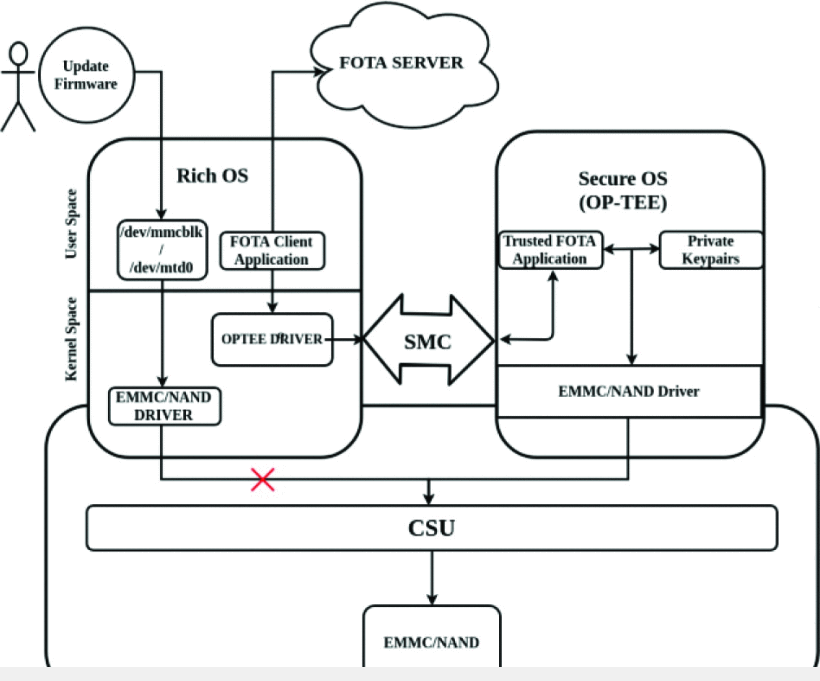
\includegraphics[width=0.5\linewidth]{figures/Architectuur secure updates.png}
    \caption{Architectuur voor de secure updates}
    \label{fig:secureUpdateArchitecture}
\end{figure}
Zie \ref{fig:secureUpdateArchitecture}, bron = link blabla.\\
Secure server (FOTA server) levert de firmware files.\\
TEE heeft geen network access dus NW OS doet download.\\
Nu zijn er 2 applications: "FOTA application" in NW en "trusted application" in SW. Deze communiceren via SMC (Secure Monitor Call).\\
\\
Dus, "Host application"(FOTA appl.) in NW doet download over secure channel met FOTA server. Gebruikt dan de OP-TEE driver om SMC te doen naar trusted application voor signature verification. Deze RSA crypto shnitzel gebeurt in TEE waar private keys zitten.\\ 
Als geverified, schrijft trusted application de firmware file naar flash via flash drivers (NW heeft geen access naar firmware flash region).\\
De access control policies voor peripherals worden onderhouden door CSU (Central Security Unit). E.g. enkel SW heeft toegang tot de EMMC / NAND waar firmware gestored wordt, CSU blockt calls van NW.\\
\\
Sectie 4: Implementatie. 
Deze paper gebruikt ARM Cortex A7, Linux in NW, OP-TEE in SW, U-Boot als bootloader. \\
Zie andere figuur in de paper voor flow, Trusted Application (TA) wordt pas ingeladen na download van nieuwe firmware. Dus flow is Bootloader start -> Bootloader laadt OP-TEE (SW) -> OP-TEE start Linux (NW) -> FOTA (Host application in NW) wordt geinitialiseerd en checkt of firmware update available is. Als nee, niks (wacht tot een update komt). Als ja -> FOTA application in NW download de firmware van de Secure server -> FOTA application initialiseert de Trusted Application in SW via call (SMC) met UUID voor deze specifieke Trusted Application) -> TA verifieert, schrijft naar EMMC / NAND flash \dots.\\
Bij inladen van de TA in SW, doen we ook validations vd authenticity etc van de TA eerst. = extra security.\\
\\
Dit is allemaal zeer interessant en nuttig voor basic implementatie in onze thesis, maar is andere richting dan wat wij willen zoeken. \\
In deze implementatie, wat als een NW application (zeg Bad Application) onze device DoS't door de network stack in de NW hele tijd bezig te houden?\\
Priority based preemption? -> Application in NW heeft somehow max priority, wat nu? Geen FOTA updates mogelijk?\\
\section{Secure FOTA updates for IoT: survey, challenges and discussions}
\url{https://www.sciencedirect.com/science/article/pii/S2542660522000142}//
\subsection{Intro en Background}
IoT heeft slechte security want security niet zo profitable als eerst zijn.\\
Veel zero-day attacks.\\
Daarom is FOTA zo belangrijk, om deze exploits snel te fixen.\\
In deze paper: Basically beschrijving van huidige landschap (security mechanisms, threats, solutions).\\
Idk paper praat wel veel uit standpunt van ISP
\\
Background:\\
New classification voor embedded devices blabla\\
Secure element is zeer belangrijk om een trusted environment te bekomen (elke device heeft SE waarin crypto shit zit om device te authenticaten etc, malicious devices kunnen uit onze trusted environment gepingeld worden). (Dit is TEE btw, e.g. TrustZone...)\\
Root-of-trust (verifieer de integriteit en authenticiteit vd software die geload wordt op device) establishen en verder Trust Chain uitbouwen.\\
Bij TrustZone: Protect keys / certificates, dit is initial layer van RoT. Start boot van IBB en bouw chain verder uit. \\
Modes of FOTA updates: Pull en Push. Pull = device query't FOTA server periodiek, Push = server-initiated, voor devices die zeer resource-constrained zijn en niet periodiek willen / kunnen checken. Hybrid mode ook mogelijk, partial FOTA updates ook cool.\\ 
FOTA update via mobile gateway: Gateway managet meerdere IoT devices. Extra concerns, zie 2.5 evt. Niet zo belangrijk.\\
\subsection{FOTA update related threats}
Beschrijving van verschillende attack types. 3 categorieen: attacks op IoT devices, op gateways en op suppliers/manufacturers. Vooral geinteresseerd in attacks op IoT devices zelf voor deze. \begin{quote}
    Since the IoT devices are the weakest node in the update process, the attackers will mainly try to exploit their constraints in order
to infiltrate the local network of the user for malicious purposes. In this section, the attacks targeting these devices are highlighted.
The ‘‘Rollback attack’’: the hacker re-sends a valid but old firmware version to the devices [2]. ‘‘Mismatched firmware’’: the
attacker sends this time a valid firmware but for a different type of IoT device, which will lead to the dysfunction of the device. Thus,
the devices become unavailable [18]. Another attack targets the very constrained devices that are most of the time in sleep mode, this
attack can be called ‘‘Offline update attack’’. Since some IoT devices are most of the time offline, they may have missed a couple of
firmware updates. In this case, the attacker sends a newer version than the one installed in the devices but still not the latest version.
This newer version may still have some unpatched vulnerabilities, that can be exploited [18]. ‘‘Repeated update requests attack‘‘:
can be seen as a kind of DoS attack where the malicious peer sends as many as possible new FoTA update requests either with
valid or invalid firmware. It leads the IoT device to check the integrity and the authenticity of the firmware each time. This attack
provokes the unavailability of the IoT device and extra power consumption, which is problematic for the battery-powered ones.
‘‘Device cloning attack‘‘: the attacker replicates some IoT devices so that only the cloned one will be updated and not the original
devices. In this case, the attacker will simply remove the cloned devices from the network and will try to exploit the unpatched
devices. ‘‘Non-ephemeral keys attack’’: in this case, the attacker tries to deduce the asymmetric key pair from all the exchanges
that have been done between the IoT device and the other entities, in particular since the IoT device will rarely renegotiate a new
pair of keys. The attacker can then forge a signature on a rogue update [18]. ‘‘Unchanged default password’’: is not a particular
problem for IoT but for all the devices where the default password was never changed, and where it can be the same for all devices
of the same model manufactured by the same manufacturer. Hence, an attacker who possesses a similar device model can suppose
that the target has also the same password. Furthermore, a weak password can be easy to guess. In both cases, an attacker may aim
to get unauthorized access to the device using the obtained password. ‘‘Firmware reverse engineering’’: is another type of process
an attacker can perform, by reverse-engineering the binaries into assembly in order to analyze the functionality and to get access
to secret data [2,19].
\end{quote}
Deze + de 2 andere categorieen versterken vgm het punt dat deze thesis nuttig is: no matter what, het is mogelijk dat onze device infected raakt. Het is dus belangrijk om, in welke situatie dan ook, de OTA update service available te hebben. \\
\subsection{Challenges}
\begin{itemize}
    \item Constraints of IoT devices: Heel zwakke IoT devices hebben mss niet eens capabilities voor authenticity checks (crypto).
    \item Security \& privacy: Integrity en authenticity van de firmware verifieren is belangrijk. End-to-end security mbv chain of trust en safe key-distribution system is de goal
    \item Interoperability: IoT devices zijn heterogeen, e.g. verschillende HW capabilities, verschillende communication protocols, verschillende architecturen \dots Moeilijk om standardised solution te vinden.
    \item Verschillende netwerk topologies: P2P, star, mesh \dots
    \item Establishing trust chain: Zoals eerder gezien, niet altijd mogelijk dat elk element in de chain alles kan authenticaten. Maybe 3rd party nodig die devices monitort \dots
\end{itemize}
\subsection{State of the art}
Zeeeer interessant, samenvatting en review van een hoop papers, zie hoofdstuk 5.\\
Vooral: [24] TUF, [33] ASSURED (TUF voor o.a. ARM TrustZone-M), [44] (zie 5.2.4) paper die FOTA update over LoraWAN standardiseert
\section{Plaatsing van ons probleem}
We gebruiken \hyperlink{https://www.enisa.europa.eu/sites/default/files/publications/ENISA\%20Report\%20-\%20Guidelines\%20for\%20Securing\%20the\%20Internet\%20of\%20Things.pdf}{ENISA guidelines for securing the IoT}. \\
Deze thesis behandelt 3.3: Nefarious activity/abuse, en meer specifiek Malware insertion. 
\begin{quote}
    Attackers are presented with the opportunity to insert malicious software
whose main objective is to provide illicit access or any other functionality
that goes against the intended usage of the system. Insecure update
mechanisms and poisoned update services are prime examples of such
opportunities for malware injection. IoT gateways are especially relevant in
this context; these are functional devices that are commonly found in IoT
architectures, but can also function as a threats source. IoT gateways
usually have a supporting role in the scope of security requirements, they
are, however, an avenue to compromise IoT devices for a malicious actor,
providing access into trusted networks and a method to acquire data from
supported constrained devices.
\end{quote}
Ook 3.5: Unintentional damage or loss of information. Meer specifiek Compromise of network \begin{quote}
    Systems that are necessary for the control of supply chain processes and
exist in a network could become compromised without the proper QoS or
firewall policies. These assets could be weaponized to orchestrate, for
example, large scale Denial of Service (DoS) attacks, or to degrade the
operation of the supply chain. Those that have access to the Internet are
the most vulnerable, although isolated internal networks are also at risk
from insider attacks.
\end{quote}
en Failure of recovery mechanics \begin{quote}
    Due to an attack, the system (and the device) is not able to be recovered
impacting functionality and security. During the lifecycle of an IoT device,
several assets (firmware, configuration, credentials) might need to be
updated. Chain of trust must be considered since depending the asset to
be updated (impacted), different mechanisms must be used. The recovery
plan must define which mechanism and which process must be followed to
fix any potential situation that might compromise the service and the
security of the device. Depending the level of criticality and the element of
the chain that is compromised, the mechanisms must be one or other. This
is a critical process in which the security of the device and the system can
be compromised.
\end{quote}
evt ook undetected software or hardware disruptions of the devices \begin{quote}
    Systems related in any fashion to the operation of the supply chain should
ideally be extensively monitored for an early detection of hardware of
software issues. A more proactive approach on detection usually results in
a reduced number of disruptions to the supply chain, especially when
compared with reactive measures.
\end{quote}
Punt van deze sectie is om deze 3.3 te plaatsen in wijdere context van IoT vulnerabilities.\\
\\
There is a lot to be said and done about security in the IoT sector. This thesis is not trying to tackle all the problems at once \dots
\\
Er is een hele IoT supply chain (zie ENISA guidelines), op elke stap kan iets fout gaan. Enkel security die OTA updates authenticate bv is niet genoeg, het is altijd mogelijk dat iets binnenslipt en bv onze comms DoS't. \\
Dus de thesis goals / research questions zijn nog steeds relevant IMO.\\

\section{Thesis outline}
Research question: How can we use a TEE in an IoT device to create a split architecture that guarantees the availability of OTA updates in the case of a possibly compromised Normal World, while minimizing the performance loss? 
\section{NetReach}
\url{https://ieeexplore.ieee.org/document/10628625}\\
Idee: RT scheduler toevoegen aan TrustZone en alle critical code in SW = goede availability. Issue: Network stack runt nog in NW, kan nog geDoS't worden.\\
NetReach oplossing: always available network peripheral in SW + always available network connection naar critical applications in NW.\\ 
Basically gewoon: geef NW transmission lage prioriteit.\\
In normal operation, NW network stack wordt gedeeld tussen NW en SW. Dan ook nog extra backup network connection van SW (aparte MAC en IP) .\\
\\
Verschil met deze thesis: \begin{itemize}
    \item NetReach gebruikt Armv7 A (meer computational power), wij gebruiken Arm Cortex M (meer resource-constrained, M33 specifiek)
    \item NetReach heeft backup network channel voor SW. Wij willen maar 1 shared channel 
    \item NetReach is split-driver architecture, wij moeten uitzoeken welke manier best is (fair sharing, priority based, meerdere drivers vs 1 driver in SW \dots)
    \item NetReach DoS protection door priority-based: NW tx lagere prio dan SW. Deze thesis: 
\end{itemize}
\section{Bronnen}
Building a secure system using TrustZone technology: \url{https://www.google.com/url?sa=t&source=web&rct=j&opi=89978449&url=https://documentation-service.arm.com/static/5f212796500e883ab8e74531&ved=2ahUKEwiMyJLq_4OQAxXLVaQEHdDXNP4QFnoECAsQAQ&usg=AOvVaw1Pe2c9ygxbbg8PjsGQV9XZ}
\\
\\
Board: \url{https://www.silabs.com/development-tools/wireless/proprietary/efr32fg23-868-915-mhz-14-dbm-dev-kit?tab=techdocs}
\\
\\
Board documentation, Reference manual etc: \url{https://www.silabs.com/support/resources.p-wireless_proprietary_efr32fg23-series-2-socs}
\\
\\
Trusted firmware site, zie TF-M: \url{https://www.trustedfirmware.org/}
\\
\\
Secure Firmware Update over the Air using TrustZone: \url{https://ieeexplore.ieee.org/document/8959992}
\\
\\
ENISA guidelines for securing the IoT: \url{https://www.enisa.europa.eu/sites/default/files/publications/ENISA\%20Report\%20-\%20Guidelines\%20for\%20Securing\%20the\%20Internet\%20of\%20Things.pdf}
\\
\\
Basically state of IoT OTA update security anno mei 2022: \url{https://www.sciencedirect.com/science/article/pii/S2542660522000142}

NetReach, paper van Tom Van Eyck et al. \url{https://ieeexplore.ieee.org/document/10628625}

Dikke Armv8-M paper: \url{https://community.arm.com/cfs-file/__key/telligent-evolution-components-attachments/01-2142-00-00-00-01-27-19/ARM-Cortex-_2D00_-session-11-_2D00_-Yiu-_2D00_-Software-Development-in-ARMv8_2D00_M-Architecture.pdf}

\chapter{The First Chapter}
\label{cha:1}
A chapter is a logical unit. It normally starts with an introduction, which
you are reading now. The last topic of the chapter holds the conclusion.

\section{The First Topic of the Chapter}
First comes the introduction to this topic.

\lipsum[55]

\subsection{An item}
Please don't abuse enumerations: short enumerations shouldn't use
``\verb|itemize|'' or ``\texttt{enumerate}'' environments.
So \emph{never write}: 
\begin{quote}
  The Eiffel tower has three floors:
  \begin{itemize}
  \item the first one;
  \item the second one;
  \item the third one.
  \end{itemize}
\end{quote}
But write:
\begin{quote}
  The Eiffel tower has three floors: the first one, the second one, and the
  third one.
\end{quote}

\section{A Second Topic}
First we start with equation~\ref{eq:1} after this paragraph.
\begin{equation}
  \label{eq:1}
  A = \pi r^2
\end{equation}

\lipsum[64]

\subsection{Another item}
\lipsum[56-57]

\section{Conclusion}
The final section of the chapter gives an overview of the important results
of this chapter. This implies that the introductory chapter and the
concluding chapter don't need a conclusion.

\lipsum[66]

\chapter{The Next Chapter}
\label{cha:2}
\lipsum[77]

\section{The First Topic of this Chapter}
\lipsum[78]

\subsection{An item}
A master's thesis is never an isolated work. This means that your text must
contain references. On-line documents\cite{wiki} as well as
books\cite{pratchett06:_good_omens} can be referenced.

Usually a text also contains inline formulas (\(\sin^2\eta + \cos^2\eta = 1\))
or formulas as separate equations.
\begin{equation}
  \sigma(t) = \frac{1}{\sqrt{2\pi}} \int_0^t e^{-x^2/2} dx 
\end{equation}


\section{Figures}
Figures are used to add illustrations to the text. The \fref{fig:logo} shows
the KU~Leuven logo as an illustration.
\begin{figure}
  \centering
  
\includegraphics{logokuleng-en}
  \caption{The logo of the Faculty of Engineering Science.}
  \label{fig:logo}
\end{figure}

\section{Tables}
Tables are used to present data neatly arranged. A table is normally
not a spreadsheet! Compare \tref{tab:wrong} en \tref{tab:ok}: which table do
you prefer?

\begin{table}
  \centering
  \begin{tabular}{||l|lr||} \hline
    gnats     & gram      & \$13.65 \\ \cline{2-3}
              & each      & .01 \\ \hline
    gnu       & stuffed   & 92.50 \\ \cline{1-1} \cline{3-3}
    emu       &           & 33.33 \\ \hline
    armadillo & frozen    & 8.99 \\ \hline
  \end{tabular}
  \caption{A table with the wrong layout.}
  \label{tab:wrong}
\end{table}

\begin{table}
  \centering
  \begin{tabular}{@{}llr@{}} \toprule
    \multicolumn{2}{c}{Item} \\ \cmidrule(r){1-2}
    Animal    & Description & Price (\$)\\ \midrule
    Gnat      & per gram    & 13.65 \\
              & each        & 0.01 \\
    Gnu       & stuffed     & 92.50 \\
    Emu       & stuffed     & 33.33 \\
    Armadillo & frozen      & 8.99 \\ \bottomrule
  \end{tabular}
  \caption{A table with the correct layout.}
  \label{tab:ok}
\end{table}

\section{Lorem Ipsum}
This section is added to check headers and footers. So this chapter must at
least contain three pages. To make sure that we get the required amount,
the \textsf{lipsum} package isn't used but the text is put directly in the
text.

\subsection{Lorem ipsum dolor sit amet, consectetur adipiscing elit}
Sed nec tortor id felis tristique sodales. Nulla nec massa eu dui fermentum
tincidunt. Integer ullamcorper ante eget eros posuere faucibus. Nam id
ligula ut augue pulvinar vulputate id at purus. Aenean condimentum tortor
eu mi placerat eget eleifend massa mollis. Nam est mi, sagittis quis
euismod eget, sagittis in nibh. Proin elit turpis, aliquam et imperdiet
sed, volutpat eu turpis.

Pellentesque vel enim tellus, vitae egestas turpis. Praesent malesuada elit
non nisi sollicitudin non blandit lacus tincidunt. Morbi blandit urna at
lectus ornare laoreet. Suspendisse turpis diam, lobortis dictum luctus
quis, commodo at lorem. Integer lacinia convallis ultricies. Sed quis augue
neque, eu malesuada arcu. Nullam vehicula, purus vitae sagittis pulvinar,
erat eros semper massa, eu egestas nibh erat quis magna. Cras pellentesque,
nisl eu dapibus volutpat, urna augue ornare quam, quis egestas lectus nulla
a lectus.

Vivamus dictum libero in massa cursus sed vulputate eros imperdiet. Donec
lacinia, libero ac lobortis egestas, nibh dui ornare arcu, luctus porttitor
velit massa sit amet quam. Maecenas scelerisque laoreet diam, vitae congue
quam adipiscing vitae. Aliquam cursus nisl a leo convallis eleifend
fermentum massa porta. Nunc libero quam, dapibus dapibus molestie sit amet,
faucibus vel nunc.

\subsection{Praesent auctor venenatis posuere}
Sed tellus augue, molestie in pulvinar lacinia, dapibus non ipsum. Fusce
vitae mi vitae enim ullamcorper hendrerit eu malesuada est. Proin iaculis
ante sed nibh tincidunt vel interdum libero posuere. Vivamus accumsan metus
quis felis congue suscipit dapibus enim mattis. Fusce mattis tortor eget
ipsum interdum sagittis auctor id metus.

Integer diam lacus, pharetra sit amet tempor et, tristique non lorem.
Aenean auctor, nisi eu interdum fermentum, lectus massa adipiscing elit,
sed facilisis orci odio a lectus. Proin mi nibh, tempus quis porta a,
viverra quis enim. In sollicitudin egestas libero, quis viverra velit
molestie eget. Nulla rhoncus, dolor a mollis vestibulum, lacus elit semper
nisi, nec sollicitudin sem urna eu magna. Nunc sed est urna, euismod congue
mi.

\subsection{Cras vulputate ultricies venenatis}
Vivamus eros urna, sodales accumsan semper vel, lobortis sit amet mauris.
Etiam condimentum eleifend lorem, ullamcorper ornare lectus aliquet vitae.
Praesent massa enim, interdum sit amet semper et, venenatis ut elit.
Quisque faucibus, quam ac lacinia imperdiet, nulla neque elementum purus,
tempus rutrum justo massa porta sapien. Vestibulum ante ipsum primis in
faucibus orci luctus et ultrices posuere cubilia Curae; Sed ultrices
interdum mi, et rhoncus sapien rutrum sed.

Duis elit orci, molestie quis sollicitudin sed, convallis non ante.
Maecenas tincidunt condimentum justo, et ultricies leo tristique vitae.
Vestibulum quis quam non lectus dapibus eleifend a vitae nibh. Nam nibh
justo, pharetra quis iaculis consequat, elementum quis justo. Etiam mollis
lacinia lacus, nec sollicitudin urna lobortis ac. Nulla facilisi.

Proin placerat risus eleifend erat ultricies placerat. Etiam rutrum magna
nec turpis euismod consectetur. Phasellus tortor odio, lacinia imperdiet
condimentum sed, faucibus commodo erat. Phasellus sed felis id ante
placerat ultrices. Aenean tempor justo in tortor volutpat eu auctor dolor
mollis. Aenean sit amet risus urna. Morbi viverra vehicula cursus.

\subsection{Donec nibh ante, consectetur et posuere id, tempus nec arcu}
Curabitur a tellus aliquet ipsum pellentesque scelerisque. Etiam congue,
risus et volutpat rutrum, est purus dapibus leo, non cursus metus felis
eget ligula. Vivamus facilisis tristique turpis, ut pretium lectus luctus
eleifend. Fusce magna sapien, ullamcorper vitae fringilla id, euismod quis
ante.

Phasellus volutpat, nunc et pharetra semper, sem justo adipiscing mauris,
id blandit magna quam et orci. Vestibulum a erat purus, ut molestie ante.
Vestibulum ante ipsum primis in faucibus orci luctus et ultrices posuere
cubilia Curae; Proin turpis diam, consequat ut ullamcorper ut, consequat eu
orci. Sed metus risus, fringilla nec interdum vel, interdum eu nunc.
Suspendisse vel sapien orci.

\subsection{Morbi et mauris tempus purus ornare vehicula}
Mauris sit amet diam quam, eget luctus purus. Sed faucibus, risus semper
eleifend iaculis, mi turpis bibendum nisl, quis cursus nibh nisl sit amet
ipsum. Vestibulum tempor urna vitae mi auctor malesuada eget non ligula.
Nullam convallis, diam vel ultrices auctor, eros eros egestas elit, sed
accumsan arcu tortor eget leo. Vestibulum orci purus, porttitor in pharetra
eget, tincidunt eget nisl. Nullam sit amet nulla dui, facilisis vestibulum
dui.

Donec faucibus facilisis mauris ac cursus. Duis rhoncus quam sed nisi
laoreet eu scelerisque massa tincidunt. Vivamus sit amet libero nec arcu
imperdiet tempor quis non libero. Sed consequat dignissim justo. Phasellus
ullamcorper, velit quis posuere vulputate, felis erat tincidunt mauris, at
vestibulum justo lectus et turpis. Maecenas lacinia convallis euismod.
Quisque egestas fermentum sapien eu dictum. Sed nec lacus in purus dictum
consequat quis vel nisl. Fusce non urna sem. Curabitur eu diam vitae elit
accumsan blandit. Nullam fermentum nunc et leo dictum laoreet. Donec semper
varius velit vel fringilla. Vivamus eu orci nunc.

\section{Conclusion}
The final section of the chapter gives an overview of the important results
of this chapter. This implies that the introductory chapter and the
concluding chapter don't need a conclusion.

\lipsum[66]

% ... en zo verder tot
\chapter{The Final Chapter}
\label{cha:n}
\lipsum[79]

\section{The First Topic of this Chapter}
\subsection{Item 1}
\subsubsection{Sub-item 1}
\lipsum[80]

\subsubsection{Sub-item 2}
\lipsum[81]

\subsection{Item 2}
\lipsum[82]

\section{The Second Topic}
\lipsum[83-85]

\section{Conclusion}
\lipsum[86-88]

\chapter{Conclusion}
\label{cha:conclusion}
The final chapter contains the overall conclusion. It also contains
suggestions for future work and industrial applications.

\lipsum[1-7]


% Indien er bijlagen zijn:
\appendixpage*          % indien gewenst
\appendix
\chapter{The First Appendix}
\label{app:A}
Appendices hold useful data which is not essential to understand the work
done in the master's thesis. An example is a (program) source.
An appendix can also have sections as well as figures and references\cite{h2g2}.

\section{More Lorem}
\lipsum[50]

\subsection{Lorem 15--17}
\lipsum[15-17]

\subsection{Lorem 18--19}
\lipsum[18-19]

\section{Lorem 51}
\lipsum[51]

% ... en zo verder tot
\chapter{The Last Appendix}
\label{app:n}
Appendices are numbered with letters, but the sections and subsections use
arabic numerals, as can be seen below.

\section{Lorem 20-24}
\lipsum[20-24]

\section{Lorem 25-27}
\lipsum[25-27]


\backmatter
% Na de bijlagen plaatst men nog de bibliografie.
% Je kan de  standaard "abbrv" bibliografiestijl vervangen door een andere.
\bibliographystyle{abbrv}
\bibliography{references}

\end{document}
